%-----------------------------------------------------------------
%	BASIC DOCUMENT LAYOUT
%-----------------------------------------------------------------
\documentclass[paper=a4, fontsize=12pt, twoside=semi, abstracton, listof=totoc, toc=left]{scrartcl}
\usepackage[T1]{fontenc}
\usepackage[utf8]{inputenc}
\usepackage{lmodern}
\usepackage{slantsc}
\usepackage{microtype}
\usepackage[british]{babel}
% \usepackage[backend=bibtex, style=phys, sorting=none, citestyle=authoryear, maxbibnames=3, maxcitenames=2]{biblatex}
\usepackage[backend=bibtex, style=trad-abbrv, sorting=none, maxbibnames=3, maxcitenames=2]{biblatex}
\addbibresource{OpenData.bib}
\makeatletter
	\def\blx@maxline{77}
\makeatother

% Sectioning layout
\addtokomafont{sectioning}{\normalfont\scshape}
\usepackage{tocstyle}
\usetocstyle{standard}
\renewcommand*\descriptionlabel[1]{\hspace\labelsep\normalfont\bfseries{#1}}
\usepackage[titletoc]{appendix}

% Empty pages
\usepackage{etoolbox}
% \pretocmd{\toc}{\cleardoubleevenemptypage}{}{}
% \pretocmd{\section}{\cleardoubleevenemptypage}{}{}
\pretocmd{\part}{\cleardoubleevenemptypage\thispagestyle{empty}}{}{}
\renewcommand\partheadstartvskip{\clearpage\null\vfil}
\renewcommand\partheadmidvskip{\par\nobreak\vskip 20pt\thispagestyle{empty}}

% Paragraph indentation behaviour
\setlength{\parindent}{0pt}
\setlength{\parskip}{0.3\baselineskip plus2pt minus2pt}
\newcommand{\sk}{\medskip\noindent}

% Fancy header and footer
\usepackage{fancyhdr}
\pagestyle{fancyplain}
\fancyhead[LO]{\thepage}
\fancyhead[CO]{}
\fancyhead[RO]{\nouppercase{\mytitle}}
\fancyhead[LE]{\nouppercase{\rightmark}}
% \fancyhead[LE]{\nouppercase{\leftmark}}
\fancyhead[CE]{}
\fancyhead[RE]{\thepage}
\fancyfoot{}
\renewcommand{\headrulewidth}{0.3pt}
\renewcommand{\footrulewidth}{0pt}
\setlength{\headheight}{13.6pt}

%-----------------------------------------------------------------
%	MATHS AND SCIENCE
%-----------------------------------------------------------------
\usepackage{amsmath,amsfonts,amsthm,amssymb}
\usepackage{xfrac}
\usepackage[a]{esvect}
\usepackage{chemformula}
\usepackage{graphicx}

\usepackage[arrowdel]{physics}
	\renewcommand{\vnabla}{\vec{\nabla}}
	% \renewcommand{\vectorbold}[1]{\boldsymbol{#1}}
	% \renewcommand{\vectorarrow}[1]{\vec{\boldsymbol{#1}}}
	% \renewcommand{\vectorunit}[1]{\hat{\boldsymbol{#1}}}
	\renewcommand{\vectorarrow}[1]{\vec{#1}}
	\renewcommand{\vectorunit}[1]{\hat{#1}}
	\renewcommand*{\grad}[1]{\vnabla #1}
	\renewcommand*{\div}[1]{\vnabla \vdot \va{#1}}
	\renewcommand*{\curl}[1]{\vnabla \cp \va{#1}}
	\let\rot\curl

% SI units
\usepackage[separate-uncertainty=true]{siunitx}
% \sisetup{range-phrase = \text{--}, range-units = brackets}
\sisetup{range-phrase = \text{--}, range-units = single}
\DeclareSIPrePower\quartic{4}
	%\DeclareSIUnit\micron{\micro\metre}

% Smaller trig functions
\newcommand{\Sin}{\trigbraces{\operatorname{s}}}
\newcommand{\Cos}{\trigbraces{\operatorname{c}}}
\newcommand{\Tan}{\trigbraces{\operatorname{t}}}

% Operator-style notation for matrices
\newcommand*{\mat}[1]{\hat{#1}}

% Matrices in (A|B) form via [c|c] option
\makeatletter
\renewcommand*\env@matrix[1][*\c@MaxMatrixCols c]{%
  \hskip -\arraycolsep
  \let\@ifnextchar\new@ifnextchar
  \array{#1}}
\makeatother

% Shorter \mathcal and \mathbb
\newcommand*{\mc}[1]{\mathcal{#1}}
\newcommand*{\mbb}[1]{\mathbb{#1}}

% Shorter ^\ast and ^\dagger
\newcommand*{\sast}{^{\star}{}}
\newcommand*{\sdag}{^{\dagger}{}}

% Blackboard bold identity
\usepackage{bbm}
\newcommand*{\bbid}{\mathbbm{1}}

% Shorter displaystyle
\newcommand*{\dsp}{\displaystyle}

% Inexact differential
\newcommand{\dbar}{\mathchar'26\mkern-12mu\mathrm{d}}
\newcommand{\indd}[1]{\dbar{#1}}

% Arrows with text and cancels for developments
\newcommand{\tikzmark}[1]{\tikz[overlay,remember picture] \node (#1) {};}
\tikzset{square arrow/.style={to path={-- ++(0,-.25) -| (\tikztotarget)}}}
\usepackage{cancel}


%-----------------------------------------------------------------
%	OTHER PACKAGES
%-----------------------------------------------------------------
\usepackage{environ}

%Left numbered equations
\makeatletter
	\NewEnviron{Lalign}{\tagsleft@true\begin{align}\BODY\end{align}}
\makeatother

% Plots and graphics
\usepackage{pgfplots}
\usepackage{tikz}
\usepackage{color}
	\makeatletter
		\color{black}
		\let\default@color\current@color
	\makeatother

% Richer enumerate, figure, and table support
\usepackage{enumerate}
\usepackage[shortlabels]{enumitem}
\usepackage{float}
\usepackage{tabularx}
\usepackage{booktabs}
	%\setlength{\intextsep}{8pt}
% \numberwithin{equation}{section}
% \numberwithin{figure}{section}
% \numberwithin{table}{section}

% No indentation after certain environments
\makeatletter
\newcommand*\NoIndentAfterEnv[1]{%
	\AfterEndEnvironment{#1}{\par\@afterindentfalse\@afterheading}}
\makeatother
%\NoIndentAfterEnv{thm}
\NoIndentAfterEnv{defi}
\NoIndentAfterEnv{example}
\NoIndentAfterEnv{table}

% Misc packages
\usepackage{ccicons}
\usepackage{lipsum}
\usepackage{todonotes}
\usepackage{array}
\usepackage{multirow}

% Print DOI only if there's no URL
\renewbibmacro*{doi+eprint+url}{%
  \iftoggle{bbx:doi}
    {\iffieldundef{url}{\printfield{doi}}{}}
    {}%
  \newunit\newblock
  \iftoggle{bbx:eprint}
    {\usebibmacro{eprint}}
    {}%
  \newunit\newblock
  \iftoggle{bbx:url}
    {\usebibmacro{url+urldate}}
    {}}

%-----------------------------------------------------------------
%	SYNTAX HIGHLIGHTING
%-----------------------------------------------------------------
\usepackage[formats]{listings}
\usepackage{relsize}
\usepackage{chngcntr}

\renewcommand{\lstlistingname}{Snippet}
\renewcommand{\lstlistlistingname}{List of snippets}

\lstloadlanguages{R}
\lstdefinelanguage{Renhanced}[]{R}{%
	morekeywords={acf,ar,arima,arima.sim,colMeans,colSums,is.na,is.null,%
	mapply,ms,na.rm,nlmin,replicate,row.names,rowMeans,rowSums,seasonal,%
	sys.time,system.time,ts.plot,which.max,which.min,%
	rename,mutate,unite,select,filter,left_join,group_by,dplyr::select,%
	ggplot,aes,geom_line,geom_hline,geom_point,geom_path,geom_errorbar,%
	geom_abline,geom_smooth%
	geom_cartogram,coord_proj,scale_x_longitude, scale_y_latitude,%
	labs,guides,annotate,theme,rowwise,%
	scale_linetype_manual,scale_colour_manual,scale_x_log10,scale_y_log10,%
	attr,paste,paste0,bind_rows,str_trim,as.numeric,as.dataframe,data.frame},
	deletekeywords={c,range,step},
	alsoletter={.,_,::},
	otherkeywords = {!,!=,~,\$,*,\&,\%/\%,\%*\%,\%\%,\%>\%,<-,<<-,\% in \%}
	}

\newcommand*{\inline}{\lstinline[basicstyle=\normalsize\ttfamily]}


\lstset{language=Renhanced,
		frame=tb,
		% captionpos=b,
		tabsize=2,
		% showtabs=true,
		breaklines=true,
		breakatwhitespace=true,
		basicstyle=\smaller\ttfamily,
		numbers=left,
		numberstyle=\tiny,
		numbersep=7.5pt,
		% commentstyle=\textsl,
		xleftmargin=3ex}
\lstset{escapeinside={(*}{*)}}   % for (*\ref{ }*) inside lstlistings (Scode)

%-----------------------------------------------------------------
%	THEOREMS
%-----------------------------------------------------------------
\usepackage{thmtools}

% Theroems layout
\declaretheoremstyle[
	spaceabove=6pt, spacebelow=6pt,
	headfont=\normalfont,
	notefont=\mdseries, notebraces={(}{)},
	bodyfont=\small,
	postheadspace=1em,
]{small}

\declaretheorem[style=plain,name=Theorem,qed=$\square$,numberwithin=section]{thm}
\declaretheorem[style=plain,name=Corollary,qed=$\square$,sibling=thm]{cor}
\declaretheorem[style=plain,name=Lemma,qed=$\square$,sibling=thm]{lem}
\declaretheorem[style=definition,name=Definition,qed=$\blacksquare$,numberwithin=section]{defi}
\declaretheorem[style=definition,name=Example,qed=$\blacktriangle$,numberwithin=section]{example}
\declaretheorem[style=small,name=Proof,numbered=no,qed=$\square$]{sproof}

%-----------------------------------------------------------------
%	ELA MOTHERFUCKING GEMINADA
%-----------------------------------------------------------------
\def\xgem{%
	\ifmmode
		\csname normal@char\string"\endcsname l%
	\else
		\leftllkern=0pt\rightllkern=0pt\raiselldim=0pt
		\setbox0\hbox{l}\setbox1\hbox{l\/}\setbox2\hbox{.}%
		\advance\raiselldim by \the\fontdimen5\the\font
		\advance\raiselldim by -\ht2
		\leftllkern=-.25\wd0%
		\advance\leftllkern by \wd1
		\advance\leftllkern by -\wd0
		\rightllkern=-.25\wd0%
		\advance\rightllkern by -\wd1
		\advance\rightllkern by \wd0
		\allowhyphens\discretionary{-}{}%
		{\kern\leftllkern\raise\raiselldim\hbox{.}%
			\kern\rightllkern}\allowhyphens
	\fi
}
\def\Xgem{%
	\ifmmode
		\csname normal@char\string"\endcsname L%
	\else
		\leftllkern=0pt\rightllkern=0pt\raiselldim=0pt
		\setbox0\hbox{L}\setbox1\hbox{L\/}\setbox2\hbox{.}%
		\advance\raiselldim by .5\ht0
		\advance\raiselldim by -.5\ht2
		\leftllkern=-.125\wd0%
		\advance\leftllkern by \wd1
		\advance\leftllkern by -\wd0
		\rightllkern=-\wd0%
		\divide\rightllkern by 6
		\advance\rightllkern by -\wd1
		\advance\rightllkern by \wd0
		\allowhyphens\discretionary{-}{}%
		{\kern\leftllkern\raise\raiselldim\hbox{.}%
			\kern\rightllkern}\allowhyphens
	\fi
}

\expandafter\let\expandafter\saveperiodcentered
	\csname T1\string\textperiodcentered \endcsname

\DeclareTextCommand{\textperiodcentered}{T1}[1]{%
	\ifnum\spacefactor=998
		\Xgem
	\else
		\xgem
	\fi#1}

%-----------------------------------------------------------------
%	DEDICATION ENVIRONMENT
%-----------------------------------------------------------------

\newenvironment{mydedication}
	{\clearpage           % we want a new page
	\thispagestyle{empty}% no header and footer
	\vspace*{\stretch{1}}% some space at the top
	\itshape             % the text is in italics
	\raggedleft          % flush to the right margin
	}
	{\par % end the paragraph
	\vspace{\stretch{3}} % space at bottom is three times that at the top
	\clearpage           % finish off the page
	}

%-----------------------------------------------------------------
%	PDF INFO AND HYPERREF
%-----------------------------------------------------------------
\usepackage{hyperref}
\hypersetup{colorlinks, citecolor=black, filecolor=black, linkcolor=black, urlcolor=black}
\usepackage{cleveref}
	\crefname{section}{\S}{\SS}
	\Crefname{section}{\S}{\SS}
	\crefname{listing}{snippet}{}

\newcommand*{\mytitle}{Crime data on the US}
\newcommand*{\mysubtitle}{Creation of a unified Data Hub using Open Data}
\newcommand*{\myauthor}{Cristian Estany \and Alfredo Hernández \and Alejandro Jiménez}
% \newcommand*{\mysupervisor}{J. Minguillón}
% \newcommand*{\mytutor}{}
\newcommand*{\myuni}{Universitat Autònoma de Barcelona}
\newcommand*{\mydate}{17th November}

\pdfstringdefDisableCommands{\def\and{and }}

\usepackage{hyperxmp}
\hypersetup{pdfauthor={\myauthor}, pdftitle={\mytitle: \mysubtitle}}

%-----------------------------------------------------------------
%	TITLE SECTION AND DOCUMENT BEGINNING
%-----------------------------------------------------------------
\newcommand{\horrule}[1]{\rule{\linewidth}{#1}}
\title{
	\normalfont
	\small \scshape{\myuni} \\ [25pt]
	\horrule{0.5pt} \\ [0.4cm]
	\huge \mytitle \\
	\Large \scshape{\mysubtitle} \\
	\horrule{2pt} \\ [0.5cm]
}
\author{\myauthor }
% \\ \footnotesize Supervised by: \mysupervisor \\ \footnotesize Academic tutor: \mytutor}
\date{\mydate}

\begin{document}

\counterwithin{lstlisting}{section}

\clearpage\maketitle
\thispagestyle{empty}
\addtocounter{page}{-1}

%-----------------------------------------------------------------
%	DEDICATION
%-----------------------------------------------------------------
% \begin{mydedication}
% 	Dedicated to RMT, Val \& the Brotherhood
% \end{mydedication}

%-----------------------------------------------------------------
%	DOCUMENT BODY
%-----------------------------------------------------------------
% \cleardoubleevenemptypage
%-----------------------------------------------------------------
%	ABSTRACT
%	!TEX root = ./../main.tex
%-----------------------------------------------------------------
\cleardoubleevenemptypage
\thispagestyle{empty}
\phantomsection
\addcontentsline{toc}{section}{Abstract}
\begin{abstract}
	% \begin{enumerate}[(a)]
	% 	\item Introduction. In one sentence, what’s the topic?
	% 	\item State the problem you tackle.
	% 	\item Summarize (in one sentence) why nobody else has adequately answered the research question yet.
	% 	\item Explain, in one sentence, how you tackled the research question.
	% 	\item In one sentence, how did you go about doing the research that follows from your big idea.
	% 	\item As a single sentence, what’s the key impact of your research?
	% \end{enumerate}
	This thesis describes the physical and statistical nature of tropical-cyclones (TC) in an environment of increasing sea surface temperature.
	The influence of global warming on the intensity of TCs is a rather controversial topic that has already been addressed in many statistical studies.
	The goal of this text is to replicate the results obtained by in \cite{Boba2004} from scratch as a learning process, to revise them using updated hurricanes track and sea surface temperature (SST) databases, and to do some new statistical analyses regarding the influence of the SST on the intensity and duration of TCs.

	Given the nature of this study, the methodology is heavily rooted in programming using a language specialised in statistical computing, along with analytical description of the maths and physics behind the TCs and the SSTs.
	Our results clearly show the effects of global warming on TC occurrence, in accordance with the results previously found by.
\end{abstract}


\pdfbookmark[1]{\contentsname}{toc}
\tableofcontents

%-----------------------------------------------------------------
%	INTRODUCTION
%	!TEX root = ./../main.tex
%-----------------------------------------------------------------
\section{Introduction}
\subsection{Summary and goals}

The arrival of Data Science has caused a great impact in many different topics and professions. From every workplace we are seeing a huge effort to adapt the usual workflow into a new, more data-driven decision making environment, in which a proper data analysis can determine the fate of any kind of professional or academic endeavour.

One of the ecosystems in which Data Science is landing and leading a new path is in criminology. A whole new topic of study is emerging from the combination of criminology and applied statistics, often called \emph{Crime Analysis}; and this topic is starting to be one of the most important tools in the decision making processes in many Public Safety Bureaus. Specifically in the United States is possible to notice an important effort from several different cities to build open data portals in which they publish police records, arrest records, distress calls, etc.

Despite this gigantic effort in organising and publishing large amounts of data, we noticed how heterogeneous these data bases were from one city to another, and how messy and unclear could be for a crime analyst to get insights from this data. For every city you can find many different data warehouses, and everyone of them stores data from various sources in some specific and usually different static structures and categories. This situation might have been sufficient in its early stages, when data were small enough, but it can get utterly messy when trying to work with data from different cities and sky-rocket the budget of a crime analysis department. This problem is not only about crime analysis departments, it is a generalised concern on \emph{Big Data}.

The \emph{Data Hub} is emerging as one of the major solutions for these Big Data issues. A stable Data Hub alleviates the costs and complications of exploratory analysis, empowering non-technical users to exploit the possibilities of data intelligence.

Our proposal in order to make this situation simpler and clearer in \emph{Crime Data Analysis} is to build a national \emph{Crime Data Hub}, in which any Police Department or any agency concerned about public safety could enter and explore uncomplicated data.

For this \emph{proof of concept} we aim to present an initial stage of what an stable Crime Data Hub could be. A Data Hub that gathers, processes, normalises, and standardises crime data from several different cities around the United States for any analysis purpose. And more importantly, this has to be done working around the computational difficulties and limitations of dealing with huge data sets.

\bigskip
Our implementation is hosted on \url{https://aldomann.shinyapps.io/crimes-hub/}, and the code and scripts developed for this project can be found on \url{https://github.com/aldomann/open-data-project}, all released under the GNU General Public License v3.0.

%-----------------------------------------------------------------
%	TOOLS AND DATA
%	!TEX root = ./../main.tex
%-----------------------------------------------------------------
\section{Tools and data}

\subsection{Data description}

Before starting mining the data and programming the scripts needed for this project, we wanted to familiarise ourselves with Crime Analysis both from an academic and a real-life point of view.

From the academic perspective, we found \cite{Boba2004} and \cite{Beardsley2014} incredibly insightful to see why data sets are structured in the way they are: Police Departments across the United States use the Uniform Crime Reporting (UCR) Program, a national standard of classifying crime uniformly that disregards state laws, providing a way to consistently count crime across the US.

On the real-life side of things, we really liked how the Chicago Tribune has a dedicated data hub on crime statistics~\cite{o:chiago-tribune} open for citizens to explore. The main feature of this data hub is the time series visualisation of crimes in the city by month (depicted in figure~\ref{fig:tribune}).

\begin{figure}[H]
	\centering
	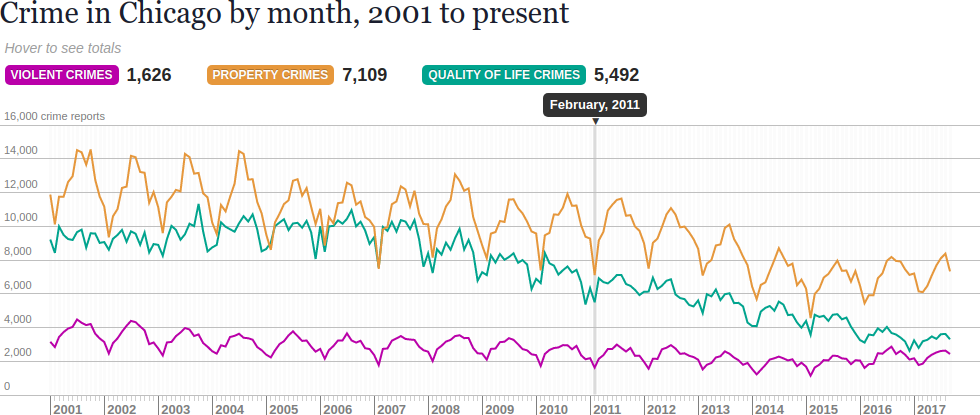
\includegraphics[width=\textwidth]{images/tribune}
	\caption{\emph{Crime in Chicago by month}, from \cite{o:chiago-tribune}}
	\label{fig:tribune}
\end{figure}

A really interesting aspect about this visualisation is that they divide crimes into three categories: (i) violent crimes, (ii) property crimes, and (iii) quality of life crimes.

We took this time series as a template of how we wanted to visualise data in our Data Hub. The main difference will be how we categorise crimes; there is some literature on how property and violent crimes are defined~\cite{Beardsley2014}, but quality of life crimes are very difficult to define. For this reason we decided to use \emph{other crimes} as a third category (we explain this categorisation process in \cref{sec:data-mining}). Apart from all this, we think it is important to include the amount of total crimes as well, as it could be really useful for an exploratory analysis.

\bigskip
Having said this, let's discuss on the data sets themselves. As we have mentioned before, our main goal is to analyse crime statistics from different cities across the US. To ensure some kind of evenly distributed sample, we chose to use data sets from 3 to 4 cities for each of the main Cultural Regions of the US (depicted in figure \ref{fig:us-map}).

\begin{figure}[H]
	\centering
	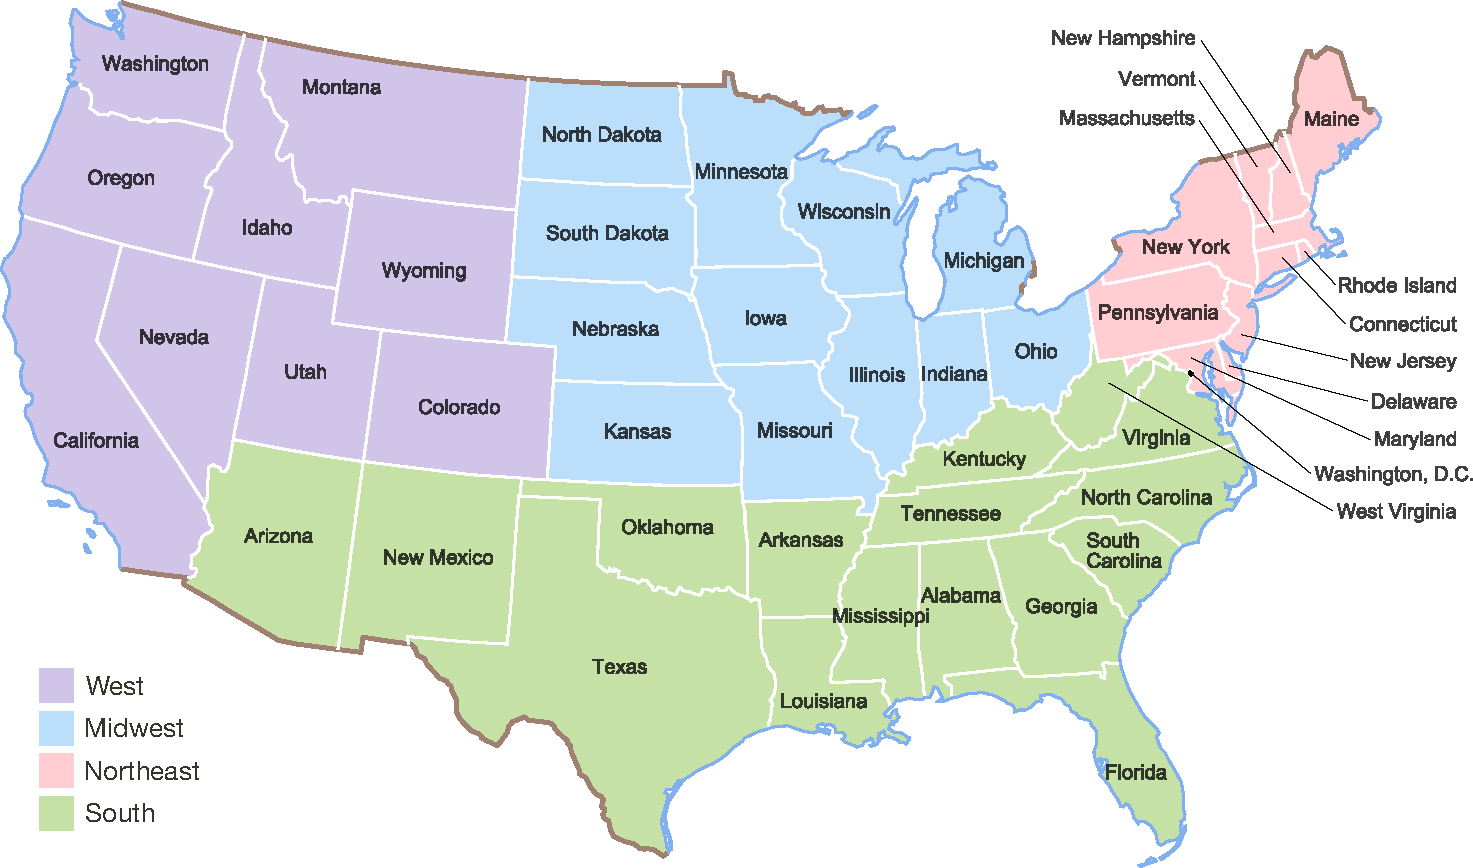
\includegraphics[width=\textwidth]{./images/us-map}
	\caption{Map of the United States divided by the four main Cultural Regions}
	\label{fig:us-map}
\end{figure}

In table \ref{tab:city-list} we can see a full description of the data sets, including geographical location, life cycle, size of the data set, and the license under which the data is released.

At a very first glance we can see how some of the data sets do not specify a license of any kind. The thing is that these databases are initially thought as a tool for Police Departments as a way to ease the report of the statistics to the FBI; the involvement of specialised professionals (that is, data scientists or crime analysts) is relatively new and they may not care about specifying a license at all\footnote{From my personal experience in the Free Software and Science communities (specially the latter), it is usual to see people that do not realise the importance of licensing and compliance.}. We can be thankful to the Police Departments, though, for making available the data in their respective city's Open Data portal. In these cases we assume they do not impose any restriction on the data and that they are Public Domain.

\begin{table}[H]
	\centering
	\label{tab:city-list}
	\resizebox{\textwidth}{!}{%
	\begin{tabular}{l l l l c l}
	\toprule
	\toprule
	City          & State          & Region    & Life Cycle            & Data Set Size & License       \\
	\midrule
	Atlanta       & Georgia        & South     & \numrange{2009}{2016} & \SI{267}{K}  & Not Specified \\
	Austin        & Texas          & South     & \numrange{2014}{2015} & \SI{159}{K}  & CC0 1.0      \\
	Baltimore     & Maryland       & Northeast & \numrange{2012}{2016} & \SI{277}{K}  & CC0 1.0      \\
	Chicago       & Illinois       & Midwest   & \numrange{2001}{2016} & \SI{6.4}{M}  & Not Specified \\
	Dallas        & Texas          & South     & \numrange{2014}{2016} & \SI{330}{K}  & ODC-By 1.0   \\
	Detroit       & Michigan       & Midwest   & \numrange{2009}{2016} & \SI{1.2}{M}  & Public Domain \\
	Los Angeles   & California     & West      & \numrange{2010}{2016} & \SI{1.6}{M}  & CC0 1.0      \\
	Metro Area    & Washington, DC & Northeast & \numrange{2008}{2016} & \SI{343}{K}  & Not Specified \\
	Minneapolis   & Minnesota      & Midwest   & \numrange{2010}{2016} & \SI{136}{K}  & CC BY-SA 3.0  \\
	New York City & New York       & Northeast & \numrange{2014}{2016} & \SI{5.6}{M}  & CC0 1.0      \\
	Philadelphia  & Pennsylvania   & Northeast & \numrange{2006}{2016} & \SI{343}{K}  & Not Specified \\
	Portland      & Oregon         & West      & \numrange{2015}{2016} & \SI{140}{K}  & Not Specified \\
	San Francisco & California     & West      & \numrange{2003}{2016} & \SI{2.1}{M}  & PDDL 1.0     \\
	Seattle       & Washington     & West      & \numrange{2009}{2016} & \SI{1.5}{M}  & CC0 1.0      \\
	\bottomrule
	\end{tabular}}
	\caption{Summary of the data we gathered during the process of building the Data Hub}
\end{table}

As a side note, we would like to clarify a bit why we focused on data sets only from the United States. The original scope of our project was to create a truly global Data Hub, gathering data from the Americas, Europe, Asia, etc. We found, alas, that although a powerful Open Data infrastructure does exist for some of the countries we checked (Spain, the Netherlands, Germany, France, the UK, Japan, Hong Kong, South Korea, etc.) the data shines for its absence. Hopefully this will change in the coming years.

The difference between the adoption ratio of Open Data in the United States vs \emph{the rest of the World} is absolutely abysmal. We believe the main reason behind this is the federal organisation of the US, which facilitates the conception of controlled and efficient policies. Another point to keep in mind is that the social and administrative concerns across the US are much more uniform than across Europe, for instance.

%-----------------------------------------------------------------
\subsection{Data mining process}\label{sec:data-mining}

One of the key points of a functional and stable Data Hub is the standardisation of its data. From one data warehouse to another we can find several different structures, categories and types of variables. So this section is about automating the \emph{data mining} process, in which we shall download and clean all the data, select the more relevant\footnote{Relevant for the purpose of this project, not in an statistical sense} variables and process them in a way so that the final output would be the same for \emph{every} data set.

\subsubsection*{Downloading the data}

As obvious as it may seem, the first thing to do is to download the raw data. Every database has its own \acr{URL} and its own origin; so this has to be treated individually for each city.

Here we show, as an example, a snippet of the code used for that purpose for San Francisco:
\begin{lstlisting}
file = "data/sanfrancisco_raw.csv"
url = "https://data.sfgov.org/api/views/tmnf-yvry/rows.csv"
download.file(url), destfile = file)
\end{lstlisting}

One particularly difficult example of this process was the city of Atlanta, for which we had the files separated by years (one file per year) and every file was formatted slightly differently. The challenge here was to merge the files together into a unified data set. For this city we developed an extra specific function for this purpose: \inline{merging_atlanta.R}

\subsubsection*{Reading \& cleaning the data}

Once we have obtained the raw data, the next step is to filter and clean it. This is a subtle point, for the process may be different from one data set to another, and the code has to be specifically tuned for every one of them.

It is usual that most of the variables (columns) in a data set are redundant or simply not necessary for our purpose, so a simple step is to select just those who are needed.  Once we have just the columns we want, the challenge is to format them in a standard way:
\begin{lstlisting}
sanfrancisco.df <- fread(file="data/sanfrancisco_raw.csv", sep = ",", header = TRUE, select = c(2,5,10,11))

sanfrancisco.df <- sanfrancisco.df %>%
	dplyr::rename(Primary.Type = `Category`) %>%
	dplyr::rename(Longitude = `X`) %>%
	dplyr::rename(Latitude= `Y`) %>%
	mutate(Date = format(as.Date(Date, format="%m/%d/%Y"), "%Y-%m-%d")) %>%
	filter(is.na(Longitude) != TRUE)
\end{lstlisting}

One particularly difficult situation in this process was found when one column was containing \inline{latitude} and \inline{longitude} in a complicated way, containing names of streets and such stuff. We used regular expressions to process the data and clean the messy structure of the variables:
\begin{lstlisting}
# Functions gathering geolocalization data
longitude <- function(x){
	a <- strsplit(x, "\\(", fixed = FALSE, perl = FALSE, useBytes = FALSE)[[1]][2]
	a <- gsub(")","", a)
	longitude <- as.numeric(strsplit(a, ",")[[1]][1])
}

latitude <- function(x){
	a <- strsplit(x, "\\(", fixed = FALSE, perl = FALSE, useBytes = FALSE)[[1]][2]
	a <- gsub(")","", a)
	latitude <- as.numeric(strsplit(a, ",")[[1]][2])
}

# Extracting longitude and latitude
detroit.df$longitude <- sapply(detroit.df$LOCATION, function(x) longitude(x) )
detroit.df$latitude <- sapply(detroit.df$LOCATION, function(x) latitude(x) )
\end{lstlisting}


\subsubsection*{Categorising Primary Types}

And then we arrive to the \emph{secret sauce} of this project. One crucial step for the purpose of this project was the classification of crimes. Doing this is quite complicated since there are a huge amount of different names used to classify the typology of crimes, often called \emph{Primary Type}. To fulfil this necessity we have created a function that contains an ever-growing dictionary of classification of crime names. This function classified all kind of crimes into three self-explanatory categories: \emph{Violent Crimes}, \emph{Property Crimes}, and \emph{Other Crimes}.

Considering the immense size of the function, the snippet below shows a small sample of the functions we use for the categorisation process:
\begin{lstlisting}[label=sn:prim_types, caption=Simplified structure of \inline{prim_types_functions.R}]
property <- c( "ARSON", "AUTO THEFT", "BIKE THEFT", "BURGLARY", ... )

violent <- c( "AGG ASSAULT", "BATTERY", "HOMICIDE", "MURDER", ... )

other <- c( "DRUNKENNESS", "FORTUNE TELLING", "TRAFFIC", ... )

# Classify primary type into Categories
find_prim_type <- function(a){
	return (ifelse(toupper(a) %in% toupper(property), "PROPERTY",
								 ifelse(toupper(a) %in% toupper(violent), "VIOLENT",
												"OTHER")))
}

# List non-classified primary types
find_new_prim_type <- function(df){
	list <- c(unique(toupper(df$Primary.Type)))
	new <- c()
	for (a in list) {
		if ( a %in% toupper(property) | a %in% toupper(violent) | a %in% toupper(other) ) {}
		else { new <- c(new, a) }
	}
	return (new)
}
\end{lstlisting}

The maintenance of this function is quite complicated, for new crime categories appear with every new data set, and then our \emph{dictionary} has to be expanded.

\subsubsection*{Summarising the data}

Now we have almost all needed variables, but the data set is still too large for being uploaded into a Data Hub to be processed in real time by the server. Now what we do is to summarise the data grouped into months. That is, we put together all crimes occurred at the same month.

\begin{lstlisting}
sanfrancisco.df <- sanfrancisco.df %>%
	group_by(Category, year = year(Date), month = month(Date)) %>%
	summarise(N=n())

\end{lstlisting}

With this, we have obtained a time series of crimes classified by categories.

A usual variable considered in typical crime analysis, is the number of crimes compared to the population of the city; obtaining the crimes per inhabitant. For this, we merged these data sets with the public access population data of every city~\cite{o:population}.

\begin{lstlisting}
# San Francisco Population ------------------------------------------------------

pop.file = "pop-data/population_sanfrancisco.csv"
sanfrancisco.pop <- fread(pop.file, sep = ";", header= TRUE, select = c(1,2))
sanfrancisco.pop$population <- as.numeric(gsub(",", "", sanfrancisco.pop$population))

sanfrancisco.df <- merge(sanfrancisco.df, sanfrancisco.pop)
sanfrancisco.df$population <- sanfrancisco.df$population
\end{lstlisting}

\subsubsection*{Deleting invalid data}

At this point we should have the data ready to be easily visualised and analysed. Before uploading the data, a careful exploration is needed to avoid unexpected surprises. By doing this, we spotted some errors or inconsistencies in the data. Usually we found a lot of gaps in the first years of the data sets, comprehensively still getting started; so we just deleted those years in order to maintain the published data consistent and reliable.

Unexpectedly, we have found a strange behaviour in the Seattle data set. There were massive holes within two years of data records. This data set is shown in our public Data Hub for the \emph{proof of concept} version, as an example of badly formatted data (this is expanded in \cref{sec:results}).

\subsubsection*{Saving the processed data set into a file}

Simple as it sounds, we just create a \inline{.csv} file containing the data set.

The success of the whole process is reflected by the fact that the initial raw data was of $\sim \SI{1}{GB}$, whilst the final output is of $\sim \SI{10}{KB}$


%-----------------------------------------------------------------
\subsection{Programming the application}

Since all the data mining process was done using R, we thought that programming the web app using the \inline{shiny} package~\cite{o:shiny} and \url{shinyapps.io}~\cite{o:shinyapps} as the platform for hosting our web app would be the most straightforward process to follow.

In short, the app consists on two parts: a \inline{ui.R} file consisting on the front end (the visual and interactive structure of the web app), and a \inline{server.R} file consisting on the back end (how the data is computed according to the user's interaction). These two files are sourced in the \inline{app.R} base file, allowing us to have a more structured and maintainable code.

In \cref{sn:app.R} we can see the whole \inline{app.R} script. As we can see, the structure is really basic and self-explanatory. The \inline{shiny.sanitize.errors = FALSE} option is used to be able to access the log files from the server, which is essential when debugging the app once it is deployed.

\begin{lstlisting}[label=sn:app.R, caption=Structure of \inline{app.R}]
## app.R ##
library(shiny)
library(markdown)

# Source UI and Server -------------------------------------

options(shiny.sanitize.errors = FALSE)

source("ui.R", local=F)
source("server.R", local=F)

shinyApp(ui, server)
\end{lstlisting}

The UI part, \cref{sn:ui.R}, is very reminiscent of what a standard program may look like. We have objects and functions that are called or used in a \emph{main function} (in this case, the \inline{ui} object):

\begin{lstlisting}[label=sn:ui.R, caption=Simplified structure of \inline{ui.R}]
# Libraries ------------------------------------------------

# UI Libs
library(shinydashboard)
library(dygraphs)

# UI -------------------------------------------------------

header <- dashboardHeader(
	title = "Crimes Data Hub"
)

cities.list <- c( "Atlanta", "Austin", ... )

sidebar <- dashboardSidebar( ... )
body <- dashboardBody( ... )

ui <- dashboardPage( skin = "purple", header, sidebar, body )
\end{lstlisting}

The server part, \cref{sn:server.R}, is probably the most difficult to work with, as you have to be really careful about how the input conditions are used to dynamically modify the data frames R is internally working with.

\begin{lstlisting}[label=sn:server.R, caption=Simplified structure of \inline{server.R}]
# Libraries ------------------------------------------------

# Server Libs
library(dplyr)
library(xts)

# Server ---------------------------------------------------

server <- function(input, output) {
	output$single.plot <- renderDygraph( { ... } )

	output$compare.plot <- renderDygraph( { ... } )
}
\end{lstlisting}

The star of the show in the app is the \inline{dygraphs} library, an R interface to the dygraphs JavaScript charting library. This allows us to:
\begin{itemize}
    \item Automatically plot \inline{xts} time series objects.
    \item Have rich interactive features including zoom/pan and series/point highlighting.
    \item Have various graph overlays in a same plot.
\end{itemize}

\bigskip

After finishing the app, we have to deal with the deployment process into the server. Using \url{http://www.shinyapps.io/} instead of a server of our own, the process is really simple. The steps to follow are, in essence:
\begin{lstlisting}
# Authenticating (only once)
rsconnect::setAccountInfo(name, token, secret)

# Deploying the app
rsconnect::deployApp("crimes-hub")
\end{lstlisting}

More details about the deployment process can be found on the documentation~\cite{o:shinyapps-docs}.

%-----------------------------------------------------------------
%	RESULTS
%	!TEX root = ./../main.tex
%-----------------------------------------------------------------
\section{Results}\label{sec:results}

Some of the motivations behind developing a Data Hub were:
\begin{itemize}
    \item Allowing users to compare crime statistics from different cities.
    \item Providing an easy method to do exploratory analysis.
\end{itemize}

In figure \ref{fig:single-chicago} we can see that the total number of crimes in Chicago seems to be decreasing at a fast rate; this could be interpreted in lots of ways. First of all, we could simply think the Chicago Police Department is doing their job, and crime is simply decreasing. But there is something important we are forgetting: property and violent crimes numbers seem to be quite stable; could this be an example of the CPD \emph{juking the stats} by registering less non-property and non-violent crimes? Could this be instead a result of the CPD having a lower records management system (RMS) budget? This is something really difficult to state for sure without having detailed budgetary and sociological information about the city; but this is definitely a starting point for a more comprehensive crime analysis.

\begin{figure}[H]
	\centering
	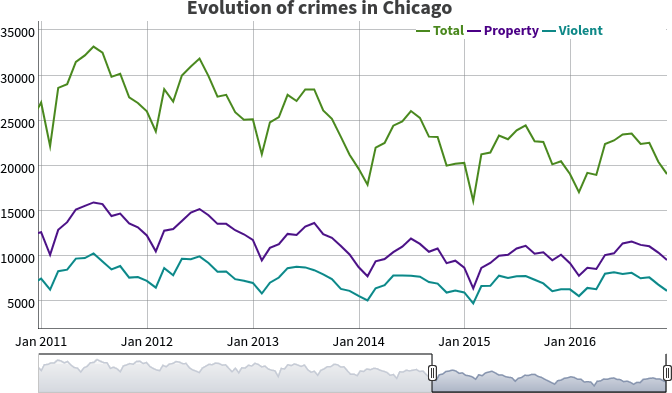
\includegraphics[width=0.8\textwidth]{images/single-chicago}
	\caption{Crime statistics in Chicago between January 2011 and December 2016}
	\label{fig:single-chicago}
\end{figure}

But this is just the analysis of one very specific city. Are more cities experiencing the same decrease in registered crimes? In figure \ref{fig:comp-base} we can see a comparison of four cities: Atlanta, Chicago, Philadelphia, and San Francisco (from the South, Midwest, Northeast, and West regions, respectively).

This time series opens a new picture on our understanding of crime statistics. It is well known that Chicago is particularly exemplary~\cite{Beardsley2014} on the early adoption of RMS systems, leading to an statistically robust data set. But how can we guess if this is the case with other cities? It is quite glaring that total crimes number by themselves are probably not the best number to analyse more than one city at the same time. For this reason we decided to give the user the ability to normalise data using two criteria: (a)~by population, depicted on figure \ref{fig:comp-pop}; and (b)~by crime mean\footnote{These ratios are widely used while comparing crime reports of different cities to study the relative time-evolution of crimes.~\cite{Boba2004}}.

\begin{figure}[H]
	\centering
	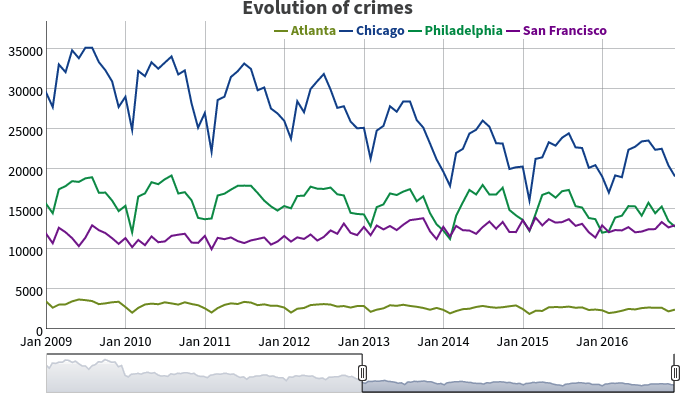
\includegraphics[width=0.8\textwidth]{images/base}
	\caption{Comparison of crime statistics between Atlanta, Chicago, Philadelphia, and San Francisco}
	\label{fig:comp-base}
\end{figure}

% \begin{figure}[H]
% 	\centering
% 	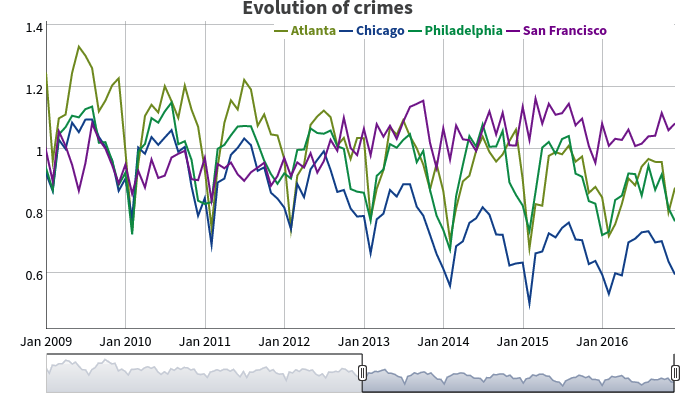
\includegraphics[width=0.8\textwidth]{images/mean}
% 	\caption{Comparison of crime statistics between Atlanta, Chicago, Philadelphia, and San Francisco; normalised by crime mean}
% 	\label{fig:comp-mean}
% \end{figure}

\begin{figure}[H]
	\centering
	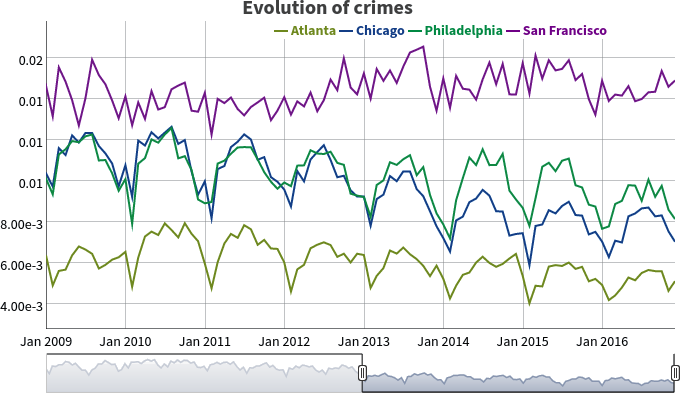
\includegraphics[width=0.8\textwidth]{images/pop}
	\caption{Comparison of crime statistics between Atlanta, Chicago, Philadelphia, and San Francisco; normalised by population}
	\label{fig:comp-pop}
\end{figure}

The differences in the three time series are remarkable. Using normalisation methods give us a much richer approach to do a qualitative comparative analysis. It is remarkable how different the West (San Francisco, Los Angeles, Portland, ...) is from the rest of the US: they are all seem to follow completely different cyclic patterns; crimes are on the rise, whilst the rest of the country seems to be improving their cities in regards to crime statistics.

Again, we could interpret these statistics in many ways. The obvious one seems to be that young and upper-class people, specially because of Hollywood and the Silicon Valley, are moving to the West coast, leading to more opportunities to commit crimes (usually property crimes). But without any proper analysis on the social predictors, this is just a wild conjecture. Quoting Rachel Boba~\cite{Boba2004},
\begin{quotation}
    \emph{All of these types of data serve a purpose in providing a picture of crime. However, depending on which data are used the picture may be very different.}
\end{quotation}


\bigskip
Last but not least, we would like to talk about Seattle (figure \ref{fig:single-seattle}). We included this city as an example of why data scientists and data analysts are required in today's world. When we first saw the data, we were quite shocked. How come there is such a huge gap of data between February 2013 and August 2014?

What we found is that for some reason, they don not have the \emph{Event Clearance Date} for most of the crimes reported in this period, but they do have the \emph{General Offense Number} (in the format \inline{YYYYN}, where \inline{YYYY} is the year \inline{N} seems to be an internal tracking code); this surely could be used by a data scientist to repopulate the missing values using data governance techniques.

\begin{figure}[H]
	\centering
	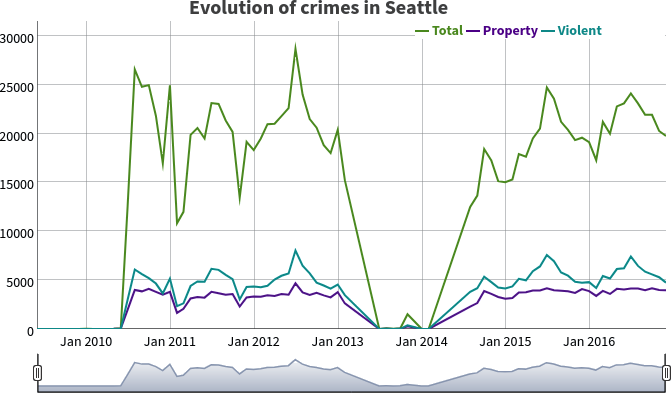
\includegraphics[width=0.8\textwidth]{images/single-seattle}
	\caption{Crime statistics in Seattle between January 2011 and December 2016}
	\label{fig:single-seattle}
\end{figure}

%-----------------------------------------------------------------
%	TEMA
%	!TEX root = ./../main.tex
%-----------------------------------------------------------------
\section{Conclusions}
% SHOULD INCLUDE:
% Limitations and future work
\lipsum[1-2]


% \begin{appendices}
% %-----------------------------------------------------------------
%	APPENDIX A
%	!TEX root = ./../main.tex
%-----------------------------------------------------------------
\section{Developed code}\label{app:code}
\renewcommand{\lstlistingname}{Script}
The code developed for this thesis is licensed under the \href{https://www.gnu.org/licenses/gpl-3.0.en.html}{GNU General Public License v3.0} and can be downloaded from \url{https://github.com/aldomann/tropical-cyclones}.

\lstinputlisting[firstline = 4, label = scr:hurdat2_base,%
	caption = \inline{hurdat2_base.R} - Base code to study the PDI of hurricane data from the National Hurricane Center (HURDAT)]%
	{code/hurdat2_base.R}
\lstinputlisting[firstline = 4, label = scr:hurdat2_pdi_base,%
	caption = \inline{hurdat2_pdi_base.R} - Base code to study the PDI probability density (DPDI)]%
	{code/hurdat2_pdi_base.R}
\lstinputlisting[firstline = 4, label = scr:hadisst_base,%
	caption = \inline{hadisst_base.R} - Base code to study the SST data from the Hadley Centre (HadISST)]%
	{code/hadisst_base.R}
\lstinputlisting[firstline = 4, label = scr:analysis_base,%
	caption = \inline{analysis_base.R} - Base code with several functions needed in \inline{main_analysis.R}]%
	{code/analysis_base.R}
\lstinputlisting[firstline = 4, label = scr:main_analysis,%
	caption = \inline{main_analysis.R} - Code to study the PDI dependence with the SST]%
	{code/main_analysis.R}
\lstinputlisting[firstline = 4, label = scr:hadcrut4_analysis,%
	caption = \inline{hadcrut4_analysis.R} - Code to study the global average temperature (from HadCRUT4)]%
	{code/hadcrut4_analysis.R}



% \end{appendices}

%-----------------------------------------------------------------
%	BIBLIOGRAPHY
%-----------------------------------------------------------------
% \nocite{Domingo2012}
\nocite{Beardsley2014}
\nocite{Wortley2008}
\nocite{McCue2015}
\nocite{Boba2004}
\nocite{ChicagoPoliceDepartment2017}

\printbibliography[heading=bibintoc]
% \setcounter{secnumdepth}{0}
% \section{References}
% \printbibliography[title={Articles}, type=article, heading=subbibliography]
% \printbibliography[title={Books}, type=book, heading=subbibliography]
% \printbibliography[title={Websites}, type=online , heading=subbibliography]
% \printbibliography[title={Other}, type=misc , heading=subbibliography]

\end{document}
